\documentclass[DIV=15,paper=letter,titlepage=true,fontsize=12pt,headings=normal,captions=nooneline]{scrartcl}
\usepackage{Style}
\usepackage[justification=centering]{caption}

\begin{document}
% !TEX root = Main.tex% !TEX root = Main.tex% !TEX root = Main.tex% !TEX root = Main.tex
\begin{center}
{\bfseries\sffamily \textls[150]{Université de Sherbrooke}\\[4pt] \textls[75]{Faculté de génie}\\\textls[75]{Département de génie électrique et de génie informatique}}
\setcounter{page}{0}
\pagenumbering{roman}
\thispagestyle{empty}
\vfill
\textbf{\huge{Rapport d'app7: Space-Invaders}}

\vfill
\textsf{\large Interfaces utilisateurs graphiques}

\vfill
\textsf{Présenté à}\\
\textsf{L'équipe professorale}

\vfill
\vfill
\vfill
\textsf{\footnotesize remis le 12 avril 2024}

\end{center}


\noindent
\rule{\linewidth}{.8pt}

\noindent
Poulin-Bergevin, Charles\hfill Pouc1302\\
Stephenne, Laurent \hfill stel2002\\

\newpage
\renewcommand*\contentsname{Table des Matières}
\tableofcontents
\newpage

\setcounter{page}{0}
\pagenumbering{arabic}

\section{Reproduction du Problème}
\subsection{Indiquer le schéma électrique}
Nous pouvons voir ci-dessous le schéma électrique de la bobine reçue. Il s'agit d'un réseau en étoile, avec une bobine centrale et trois branches de longueurs variables. La branche B est connectée à un générateur d'ondes carrées de 1 MHz. La branche A est connectée à une résistance de 50ohms. La branche C est un circuit ouvert.

\begin{figure}[H]
    \centering
    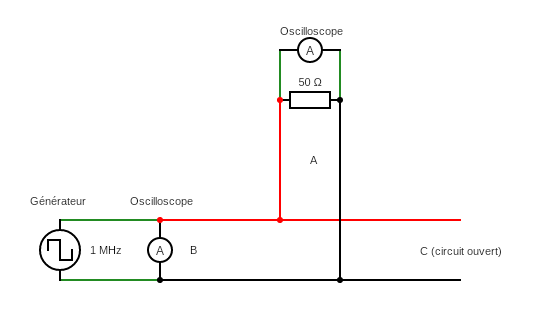
\includegraphics[width=0.7\textwidth]{images/circuit-diagram.png}
    \caption{Schéma électrique du réseau}
    \label{fig:Schema electrique}
\end{figure}

\FloatBarrier
\subsection{Comparer le signal reçu aux spécifications de la carte}
La figure suivante représente l'onde observée lorsque le signal possède une fréquence d'1MHz et qu'un des fils est resté en circuit ouvert. (voir \ref{fig:Signal à 1MHz}) La
ligne bleu représente le signal à l'entrée du circuit (connecteur du fil A). La ligne jaune représente le signal à l'extrémité du circuit
(connecteur du fil B).

\begin{figure}[H]
    \centering
    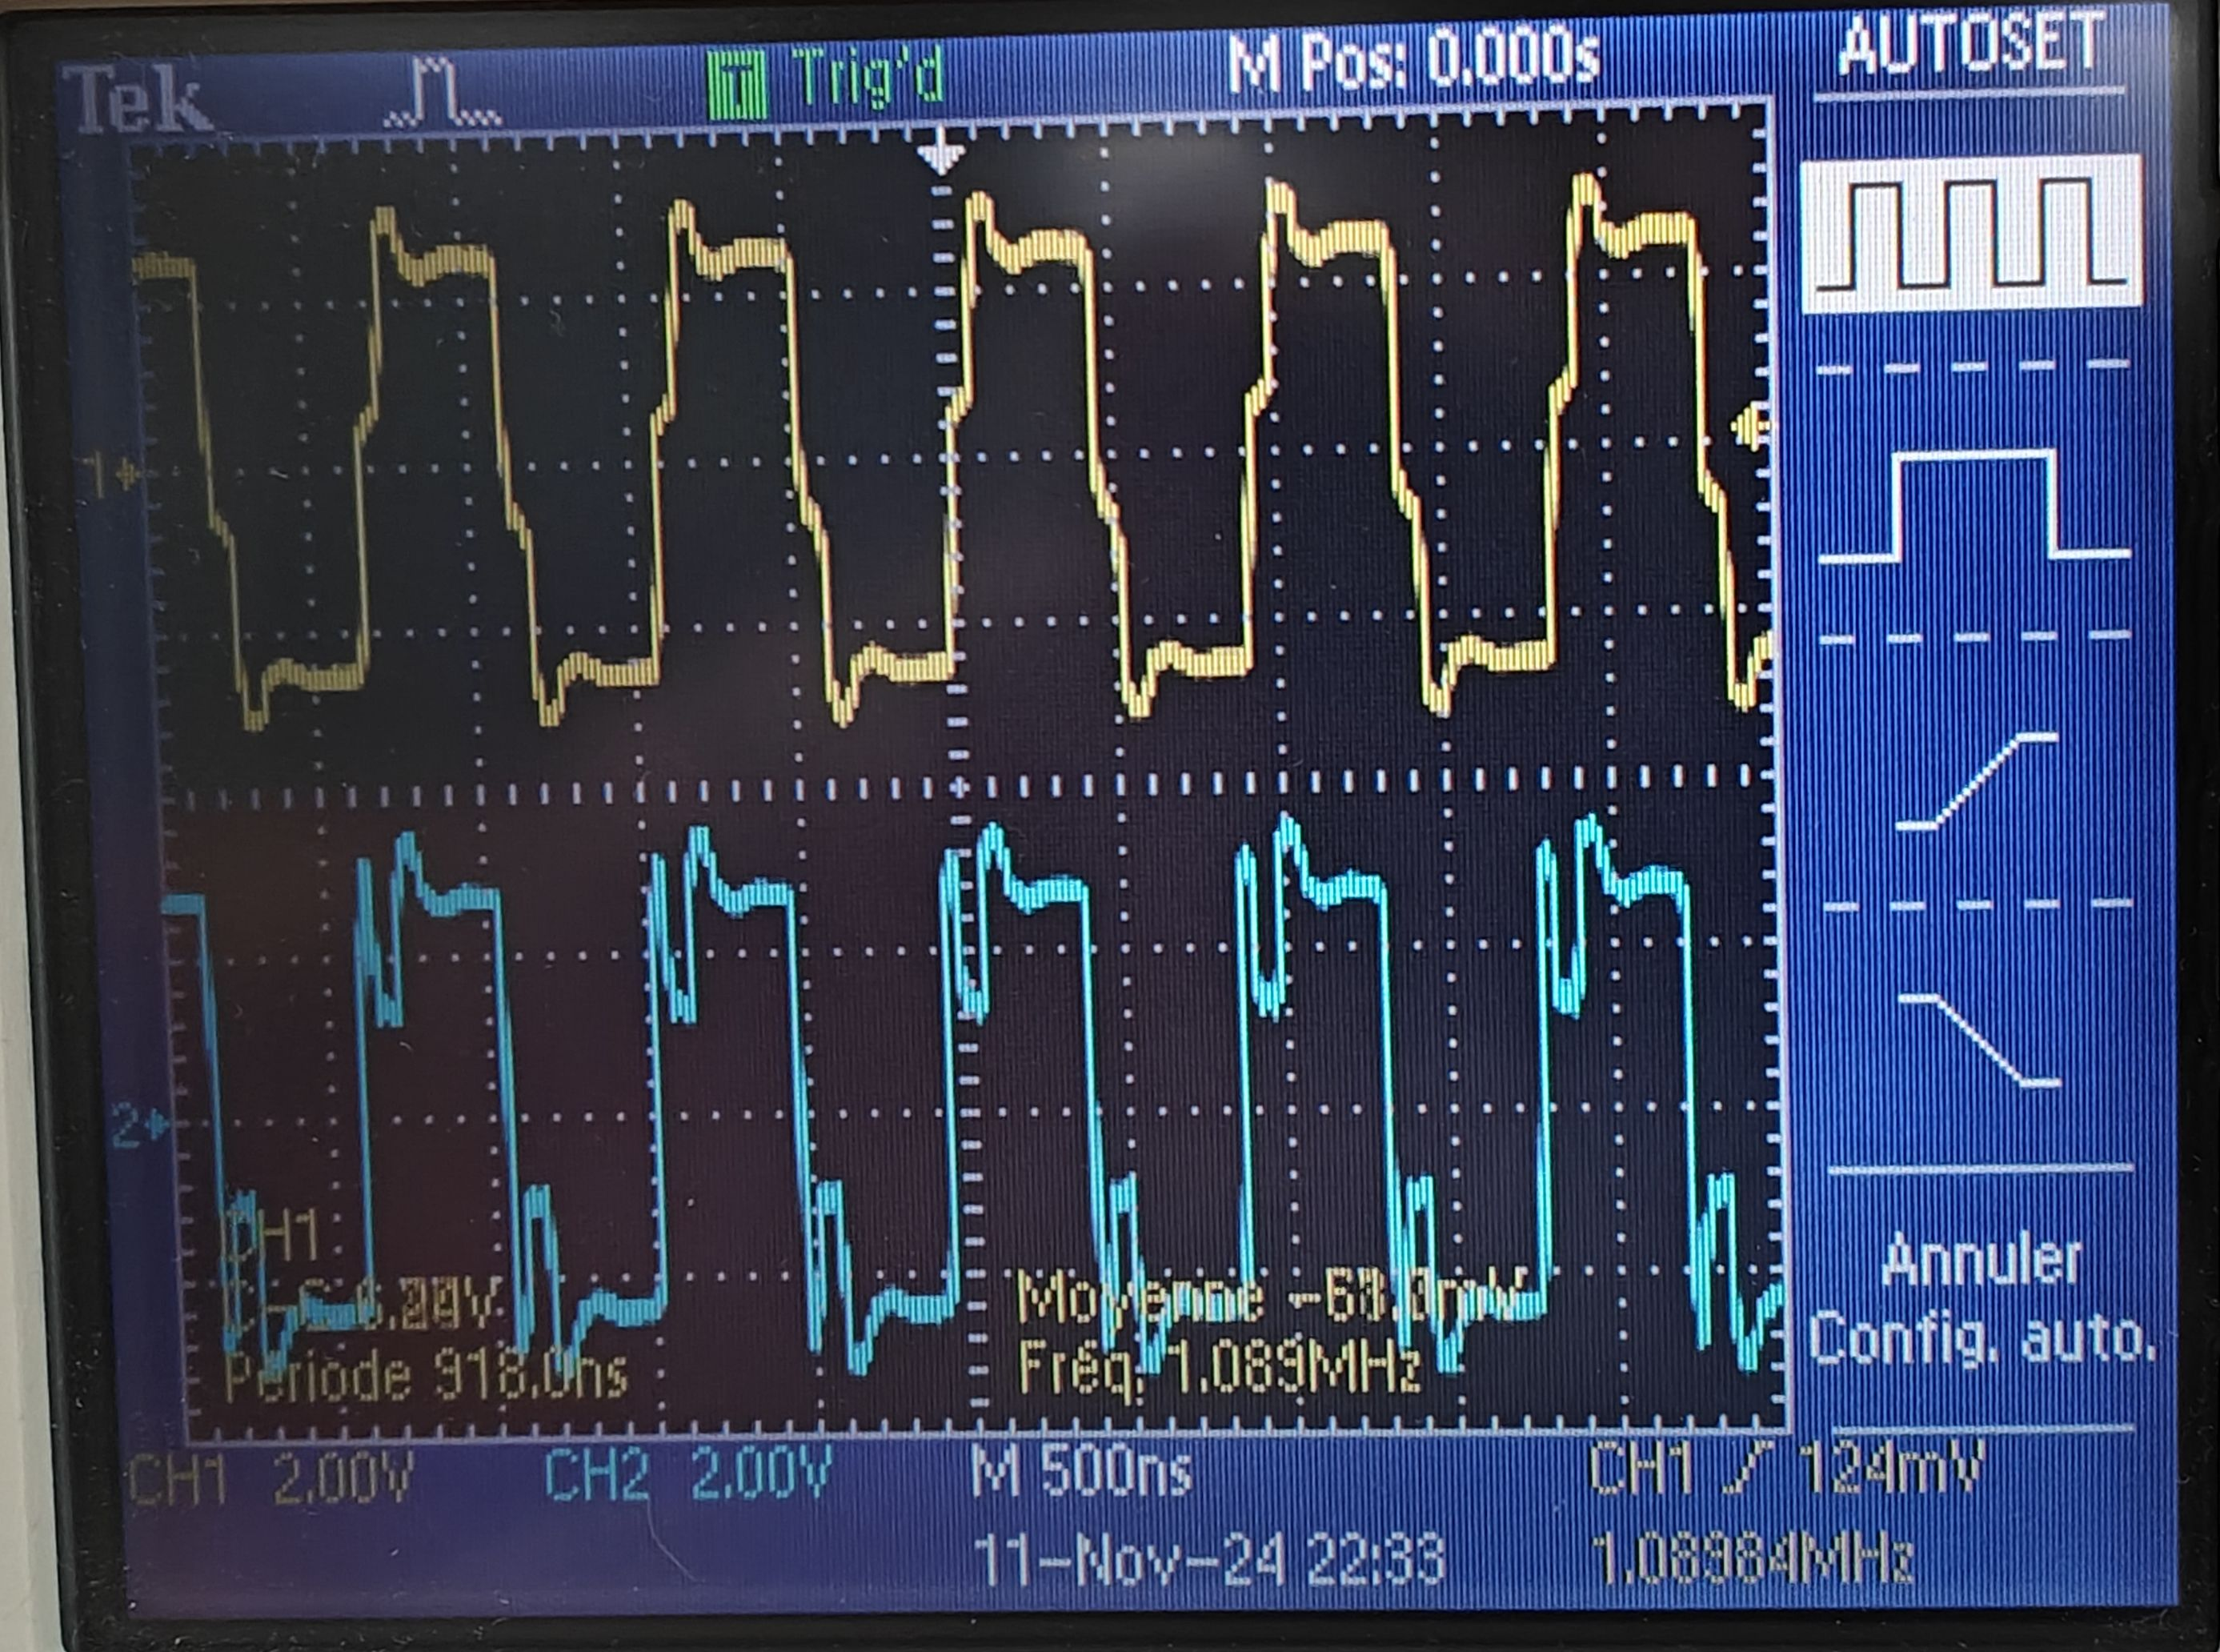
\includegraphics[width=0.7\textwidth]{images/1mhz.jpg}
    \caption{Signaux d'entrée et de sortie à 1MHz}
    \label{fig:Signal à 1MHz}
\end{figure}

On peux voir que les impulsions carrées sont déformées par la réflexion du signal sur la branche ouverte. La réflexion est aussi forte car lorsqu'un fil est laissé en circuit ouvert, sont impédance est infinie. Par contre, les impulsions ont une amplitude de plus de 2V et une durée d'environ 450ns ce qui est adéquat pour que la carte réseau les décode correctement.

\FloatBarrier

\section{Analyse temporelle}
\subsection{Identification de chaque créneau}
En observant la figure précédemment introduite: \ref{fig:Signal à 1MHz}, les conclusions suivantes peuvent être tirées: \\
\\
Lorsque l'on observe le cycle de la ligne bleu, on peut voir que juste après le début de l'émission du signal, une descente se produit lorsque
la réflection du signal se produit et revient à l'entrée du circuit. La réflexion est aussi forte car lorsqu'un fil est laissé en circuit ouvert,
le coefficient de réflection est de 1. On peut observer que la ligne jaune ne semble pas avoir les mêmes "corrections" induites par la réflection
que la ligne bleu. Cela s'explique par le fait que la réflection a l'effet inverse sur la sortie. Si l'on observe attentivement, là où l'onde est
augmenté sur la ligne bleu, elle diminue sur la ligne jaune et vice-versa, mais à une amplitude réduite aussi.

\FloatBarrier
\subsection{Explication du Problème}
 Au niveau fréquentiel, les problèmes survenants sont surtouts liés au principe de l'impédance ramenée. Cela fait, que la réflection crée des annulations
 partielles trop importantes. Cela vient diminuer l'amplitude du signal jusqu'à un point ou la carte ne peut plus lire le signal émis (amplitude
 plus basse que 0.5V). Ce phénomène se produit lorsque la longueur d'un cable est proche d'un multiple de la longeur d'onde du signal.
 Ces problèmes peuvent être rêglés en adaptant l'impédance du circuit (rajouter des fin de connections sur les fils non-utilisés), en s'assurant
 que les fils possèdent une bonne longueur selon la fréquence souhaitée, ou encore en utilisant des cables spécialisés possédants déjà l'impédance
 souhaitée.
\FloatBarrier
\subsection{Mesure par analyse temporelle des branches}

 En utilisant la formule suivante, on peut calculer la longueur du fil si l'on connait la vitesse de transmission dans notre fil et le temps de transmission:
 
 \begin{equation}
 v = \frac{\Delta X }{\Delta T} \label{eq:equation-vitesse}
 \end{equation}
 
 Donc, en utilisant les résultats suivants obtenus en prenant la mesure entre l'émission de l'onde et sa réception à l'autre extrémité du circuit
 ,comme la figure ci-dessous le démontre, On peut arriver aux résultats suivants.

 \begin{figure}[H]
    \centering
    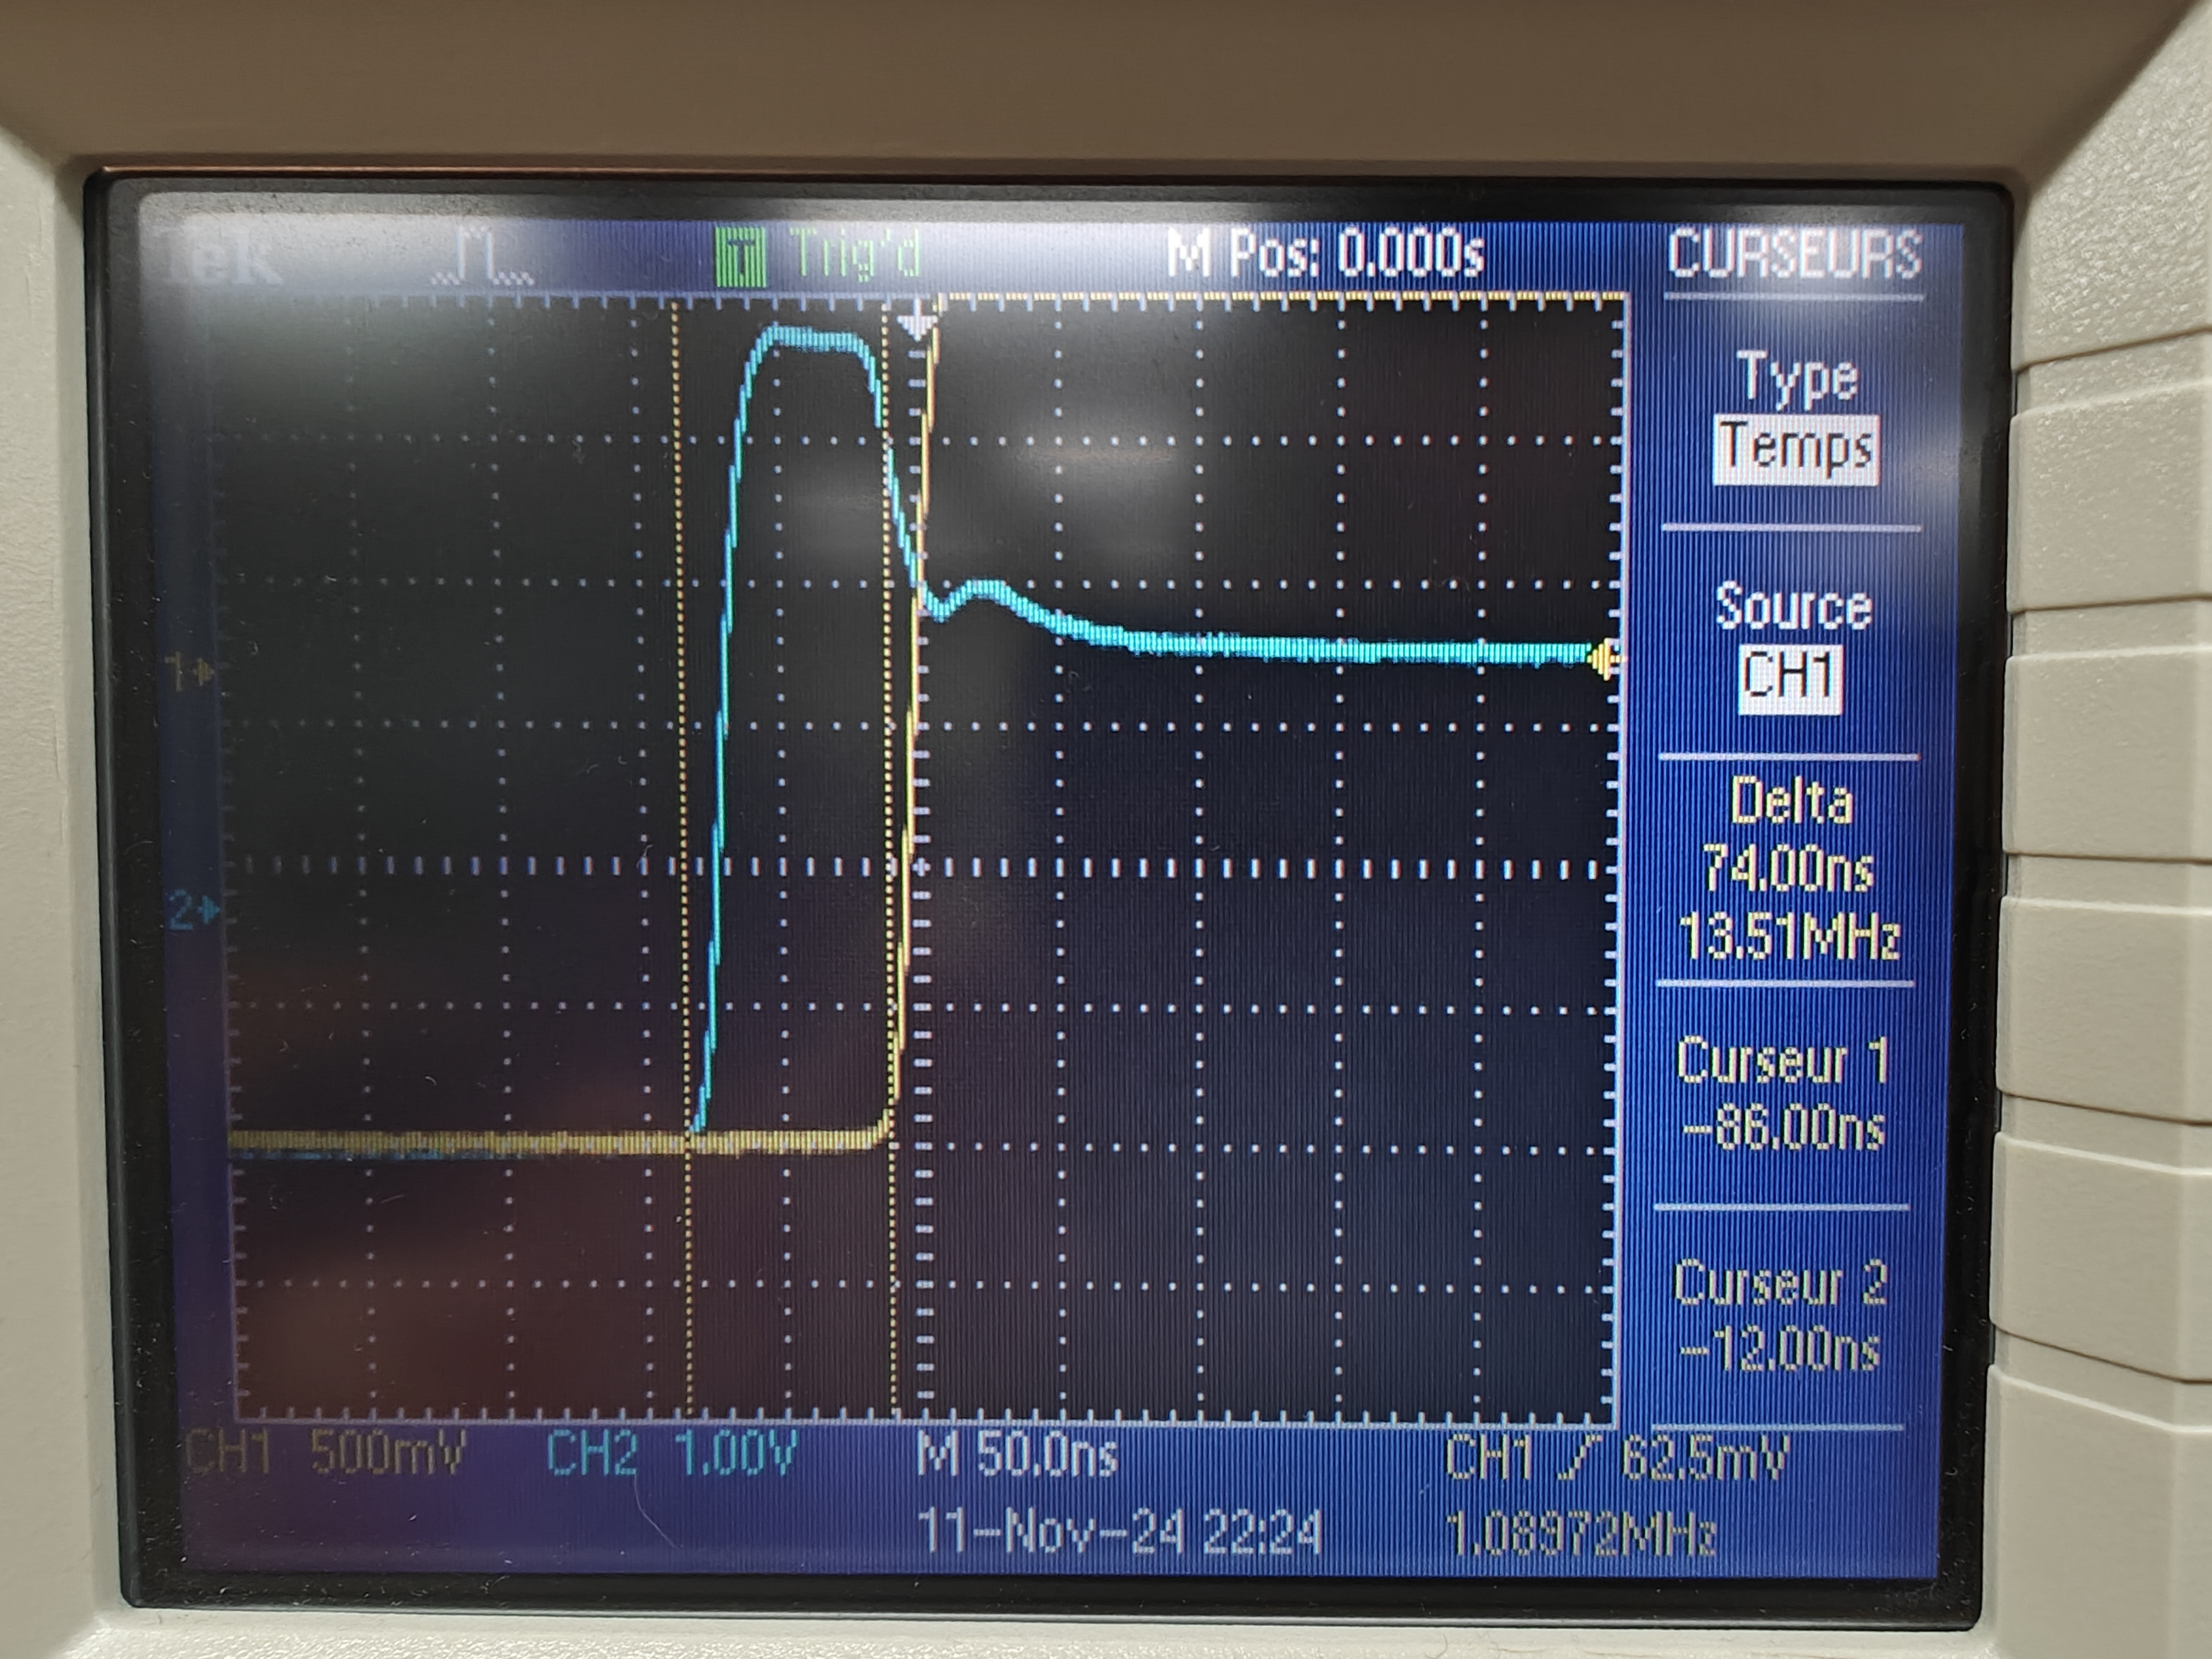
\includegraphics[width=0.7\textwidth]{images/a-b-temporel.jpg}
    \caption{Mesure temporelle du temps de réception du signal}
    \label{fig:Signal à 1MHz}
 \end{figure}


 \begin{center}
 \begin{table}[H]
 \caption{Résultats des mesures temporelles} \label{tab:tableau mesures temporel}
 \begin{tabularx}{\textwidth}{ X X X X }
    Fil d'entrée & Fil d'extrémité & Fil ouvert & Résultat (ns) \\
    \hline
    \hline
     A & B & C & 74\\
     B & C & A & 60\\
     C & A & B & 52\\
     \hline
 \end{tabularx}
 \end{table}
 \end{center}


 La vitesse de transmission assumée du fil est de 2/3 de la vitesse de la lumière, ce qui donne: 
 \begin{equation}
    2*10^8 \frac{m}{s}
    \label{vitesse-transmission}
\end{equation}

 On peut donc obtenir les résultats suivants en utilisant nos mesures et la formule de vitesse \ref{eq:equation-vitesse} on obtient 3 équations
 et 3 inconnues.

 \begin{center}
 \begin{table}[H]
 \caption{Longeurs selon les mesures temporelles} \label{tab:tableau longueur temporel}
 \begin{tabularx}{\textwidth}{ X X }
     Fil & Longueur (m) \\
     \hline
     \hline
     A & 5,9 \\
     B & 7.7 \\
     C & 4.3 \\
     \hline
 \end{tabularx}
 \end{table}
 \end{center}

\FloatBarrier


\section{Analyse fréquentielle}
\subsection{Explication du problème dans le domaine fréquentiel}
 Au niveau fréquentiel, les problèmes survenants sont surtouts liés au principe de l'impédance ramenée. Cela fait, que la réflection crée des annulations
 partielles trop importantes. Cela vient diminuer l'amplitude du signal jusqu'à un point ou la carte ne peut plus lire le signal émis (amplitude
 plus basse que 0.5V). Ce phénomène se produit lorsque la longueur d'un cable est proche d'un multiple de la longeur d'onde du signal.
 Ces problèmes peuvent être rêglés en adaptant l'impédance du circuit (rajouter des fin de connections sur les fils non-utilisés), en s'assurant
 que les fils possèdent une bonne longueur selon la fréquence souhaitée, ou encore en utilisant des cables spécialisés possédants déjà l'impédance
 souhaitée.
\FloatBarrier
\subsection{Détermination précise des longueurs des 3 branches}
Le principe d'inductance ramenée explique le fait que lorsque la longueur du fil correspond au quart de la longueur d'onde, l'onde émise se voit
presque annulée en amplitude (car réduite par sa propre réflection). Cela veut donc dire que le fil mesuré est le fil ouvert.

\begin{equation}
    L = \frac{\lambda}{4}
    \label{eq:longueur4lambda-fréquentiel}
\end{equation}

 En utilisant la formule suivante, on peut calculer la longueur du fil si l'on connait la vitesse de transmission dans notre fil et la fréquence:

\begin{equation}
\lambda = \frac{v}{F} \label{eq:equation-vitesse-fréquentiel}
\end{equation}

 on peut donc combiner les équations \ref{eq:longueur4lambda-fréquentiel} et \ref{eq:equation-vitesse-fréquentiel} et le fait que nos fréquences
 seront en MHz et que notre vitese est une constante \ref{vitesse-transmission} afin d'obtenir la simple équation suivante:

 \begin{equation}
    \begin{aligned}
        \lambda & = \frac{2*10^8}{F*10^6} \\
        L & = \frac{200}{F} / 4 \\
        L & = \frac{50}{F}
        \label{eq:equation-longueur-simple}
    \end{aligned}
 \end{equation}

 Donc, en utilisant les résultats suivants obtenus en prenant la mesure de la fréquence lorsque l'amplitude est la plus réduite possible, comme
 la figure ci-dessous le démontre, on peut arriver aux résultats suivants.

\begin{figure}[H]
   \centering
   \includegraphics[width=0.7\textwidth]{images/c-frequentiel.jpg}
   \caption{Mesure fréquentielle d'aténuation du signal}
   \label{fig:mesure-frequentiel}
\end{figure}


\begin{center}
\begin{table}[H]
\caption{Résultats des mesures fréquentielles} \label{tab:tableau mesures fréquentiel}
\begin{tabularx}{\textwidth}{ X X X X }
   Fil d'entrée & Fil d'extrémité & Fil ouvert & Résultat (MHz) \\
   \hline
   \hline
    B & C & A & 8.18\\
    C & A & B & 6.5\\
    A & B & C & 11.45\\
    \hline
\end{tabularx}
\end{table}
\end{center}

On peut donc obtenir les résultats suivants en utilisant nos mesures et la formule de vitesse \ref{eq:equation-vitesse} on obtient 3 équations
et 3 inconnues.

\begin{center}
\begin{table}[H]
\caption{Longeurs selon les mesures fréquentielles} \label{tab:tableau longueur frequentiel}
\begin{tabularx}{\textwidth}{ X X }
    Fil & Longueur (m) \\
    \hline
    \hline
    A & 6.11 \\
    B & 7.69 \\
    C & 4.40 \\
    \hline
\end{tabularx}
\end{table}
\end{center}

On peut donc voir que les mesures concordent avec celles obtenues en \ref{tab:tableau longueur temporel}
\FloatBarrier


\section{Solution du problème observé}
\subsection{Solution simple sans modifier le réseau}
 La solution simple venant rêgler les différents problèmes determinés par nos tests est de ne laisser aucun fils en circuit ouvert. Cela veut dire
 qu'il faut absolument que chaque fils aient une impédance de 50ohms à leurs bouts, que ce soit par une carte ou un simple connecteur possédant
 la bonne impédance. Cela vient rêgler les problèmes d'impédance ramenée et les problèmes de réflexion. Le 50 ohms est proposé car c'est l'impédance
 des cartes déjà utilisées.
\FloatBarrier
\subsection{Solution en remplaçant le connecteur en T}
 Le connecteur en T devrait être remplacé par un connecteur en T dont chaque connecteur possède déjà une impédance adptée, permettant ainsi
 d'annuler la réflection causée par le connecteur. De plus, comme pour la solution simple, il ne faut pas de circuits ouverts, on doit donc avoir
 une carte ou simplement une résistance rajoutée à chaque fin de connection afin d'éviter de la réflection. Le calcul suivant démontre les résistances
 nécessaire pour adapter l'impédance du connecteur en T comme expliqué précédemment.

 \begin{equation}
    \begin{aligned}
        Zl & = Zc = 50 \\
        R1 & = R2 = R3 \\
        Zl & = R1 + [(R3 + Zc) // (R2 + Zc)] \\
        Zl & = R1 + (\frac{1}{R3 + Zc} + \frac{1}{R2 + Zc})^-1 \\
        Z & = R + (\frac{2}{R + Z})^-1 \\
        Z & = R + \frac{R + Z}{2} \\
        50 & = R + \frac{R + 50}{2} \\
        25 & = R + \frac{R}{2} \\
        25 * \frac{2}{3} & = R1 \\
        R & = 16.66 \\
        \label{eq:equation-longueur-simple}
    \end{aligned}
 \end{equation}
\FloatBarrier


\section{Viabilité de la technologie}
\subsection{Problèmes à 1GHz}
Lorsqu'on augmente la fréquence du générateur d'ondes jusqu'à 10GHz, la réflection du signal est beacoup plus forte, et les signaux d'entrée et de sortie sont non reconnaissables. Les cartes réseaux ne peuvent pas décoder ces signaux, étant donnée que la longeur des impulsions est trop courte.

\FloatBarrier
\subsection{Est-ce qu'un réseau avec des centaines de clients fontcionne en full duplex?}
Il est improbable que la communication full-duplex soit possible avec une centaine de clients, surtout à haute fréquence.
En effet, la réflexion causée par une centaine de connecteurs en T ammenerait des interférences qui rendraient toute communication impossible.
Même une fois ce problème règlé, l'atténuation des signaux dans un réseau passif serait trop importante pour garder une amplitude de plus de 0.5V dans l'entiereté du réseau.
Il est donc nécessaire de trouver une autre solution pour la communication full-duplex.

\FloatBarrier


\end{document}
